\documentclass[12pt]{article}
\setlength{\oddsidemargin}{0in}
\setlength{\evensidemargin}{0in}
\setlength{\textwidth}{6.5in}
\setlength{\parindent}{0in}
\setlength{\parskip}{\baselineskip}
\usepackage{amsmath,amsfonts,amssymb}
\usepackage{graphicx}
\usepackage{enumitem}
\usepackage[]{algorithmicx}
\usepackage{amsthm}
\usepackage{fancyhdr}
\pagestyle{fancy}
\setlength{\headsep}{36pt}
\usepackage{tkz-berge}
\usetikzlibrary{positioning, automata}

\usepackage{hyperref}

\theoremstyle{remark}
\newtheorem*{solution}{Solution}

\newcommand{\makenonemptybox}[2]{%
%\par\nobreak\vspace{\ht\strutbox}\noindent
\item[]
\fbox{% added -2\fboxrule to specified width to avoid overfull hboxes
% and removed the -2\fboxsep from height specification (image not updated)
% because in MWE 2cm is should be height of contents excluding sep and frame
\parbox[c][#1][t]{\dimexpr\linewidth-2\fboxsep-2\fboxrule}{
  \hrule width \hsize height 0pt
  #2
 }%
}%
\par\vspace{\ht\strutbox}
}
\makeatother

\begin{document}

\lhead{{\bf CSCI 3104, Algorithms \\ Problem Set 7a (14 points)} }
\rhead{Name: Luna McBride \\ ID: 107607144 \\ {\bf Profs.\ Hoenigman \& Agrawal\\ Fall 2019, CU-Boulder}}
\renewcommand{\headrulewidth}{0.5pt}

\phantom{Test}

\begin{small}
\textit{Advice 1}:\ For every problem in this class, you must justify your answer:\ show how you arrived at it and why it is correct. If there are assumptions you need to make along the way, state those clearly.
\vspace{-3mm} 

\textit{Advice 2}:\ Verbal reasoning is typically insufficient for full credit. Instead, write a logical argument, in the style of a mathematical proof.\\
\vspace{-3mm} 

\textbf{Instructions for submitting your solution}:
\vspace{-5mm} 

\begin{itemize}
	\item The solutions \textbf{should be typed} and we cannot accept hand-written solutions. \href{http://ece.uprm.edu/~caceros/latex/introduction.pdf}{Here's a short intro to Latex.}
	\item You should submit your work through \href{https://www.gradescope.com/courses/59294}{\textbf{Gradescope}} only.
	\item If you don't have an account on it, sign up for one using your CU email. You should have gotten an email to sign up. If your name based CU email doesn't work, try the identikey@colorado.edu version. 
	\item Gradescope will only accept \textbf{.pdf} files (except for code files that should be submitted separately on Gradescope if a problem set has them) and \textbf{try to fit your work in the box provided}. 
	\item You cannot submit a pdf which has less pages than what we provided you as Gradescope won't allow it. 
\end{itemize}
\vspace{-4mm} 
\end{small}

\hrulefill
\pagebreak

\begin{enumerate}

    \item (1 pt) Provide a one-sentence description of each of the components of a divide and conquer algorithm.
    
    \begin{solution}
    $\newline$ Divide: splits up the problem into smaller problems, which are easier to solve than the large counterpart. $\newline \newline$ Conquer: Once small enough that smaller values do not provide much, solve the tiny problems. Otherwise, divide again. $\newline \newline$ Combine: bring the solved small problems back to the big. If all went well, the large problem is also solved now as well.
    \end{solution}
    
    \item (3 pts) Use the array $A=[2,5,1,6,7,9,3]$ for the following questions
    \begin{enumerate}
        \item (1 pt) What is the value of the pivot in the call $partition(A,0,6)$?
        
        \begin{solution}
        $\newline$ This depends on the strategy we use. However, if we assume the basic strategy is used, the pivot is the last value of the array. In this case, it would be A[6], which is 3.
        \end{solution}
        
        \item (1 pt) What is the index of that pivot value at the end of that call to $partition()$?
        
        \begin{solution}
        $\newline$ (Just some quicksort in my head guided by what I typed after this to make sure I have this right) $\newline$ 2$<3$? yes, swap(2,2). 5$<$3? no. 1$<$3? yes, swap(5,1). 6$<$3? no. 7$<$3? no. 9$<$3? no. Now at 3, so swap(5,3) (5 being after the last value less than 3).
$\newline \newline$ There are 2 values less than 3, so 3 is set at A[2] with a new array A=[2,1,3,6,7,9,5], where those to the left of 3 are less than 3 and those on the right are greater than or equal to 3.
        \end{solution}
        
        \item (1 pt) On the next recursive call to Quicksort, what sub-array does $partition()$ evaluate?
        
        \begin{solution}
        $\newline$ Quicksort has two recursive calls, typically being called on left of the pivot then on right (Though I guess you could do it right then left, but let's go with typical notation). This would mean the call would be to the left of 3 in A[0]-A[1], leaving the partition function with $partition(A,0,1)$.
        \end{solution}
        
    \end{enumerate}
	\item (4 pts) Draw the tree of recursive calls that Quicksort makes to sort the list \\${E,X,A,M,P,L,E}$ in alphabetical order. Use the last element in the sub-list in each recursive call as the pivot.
	
	\begin{solution}
        $\newline$ $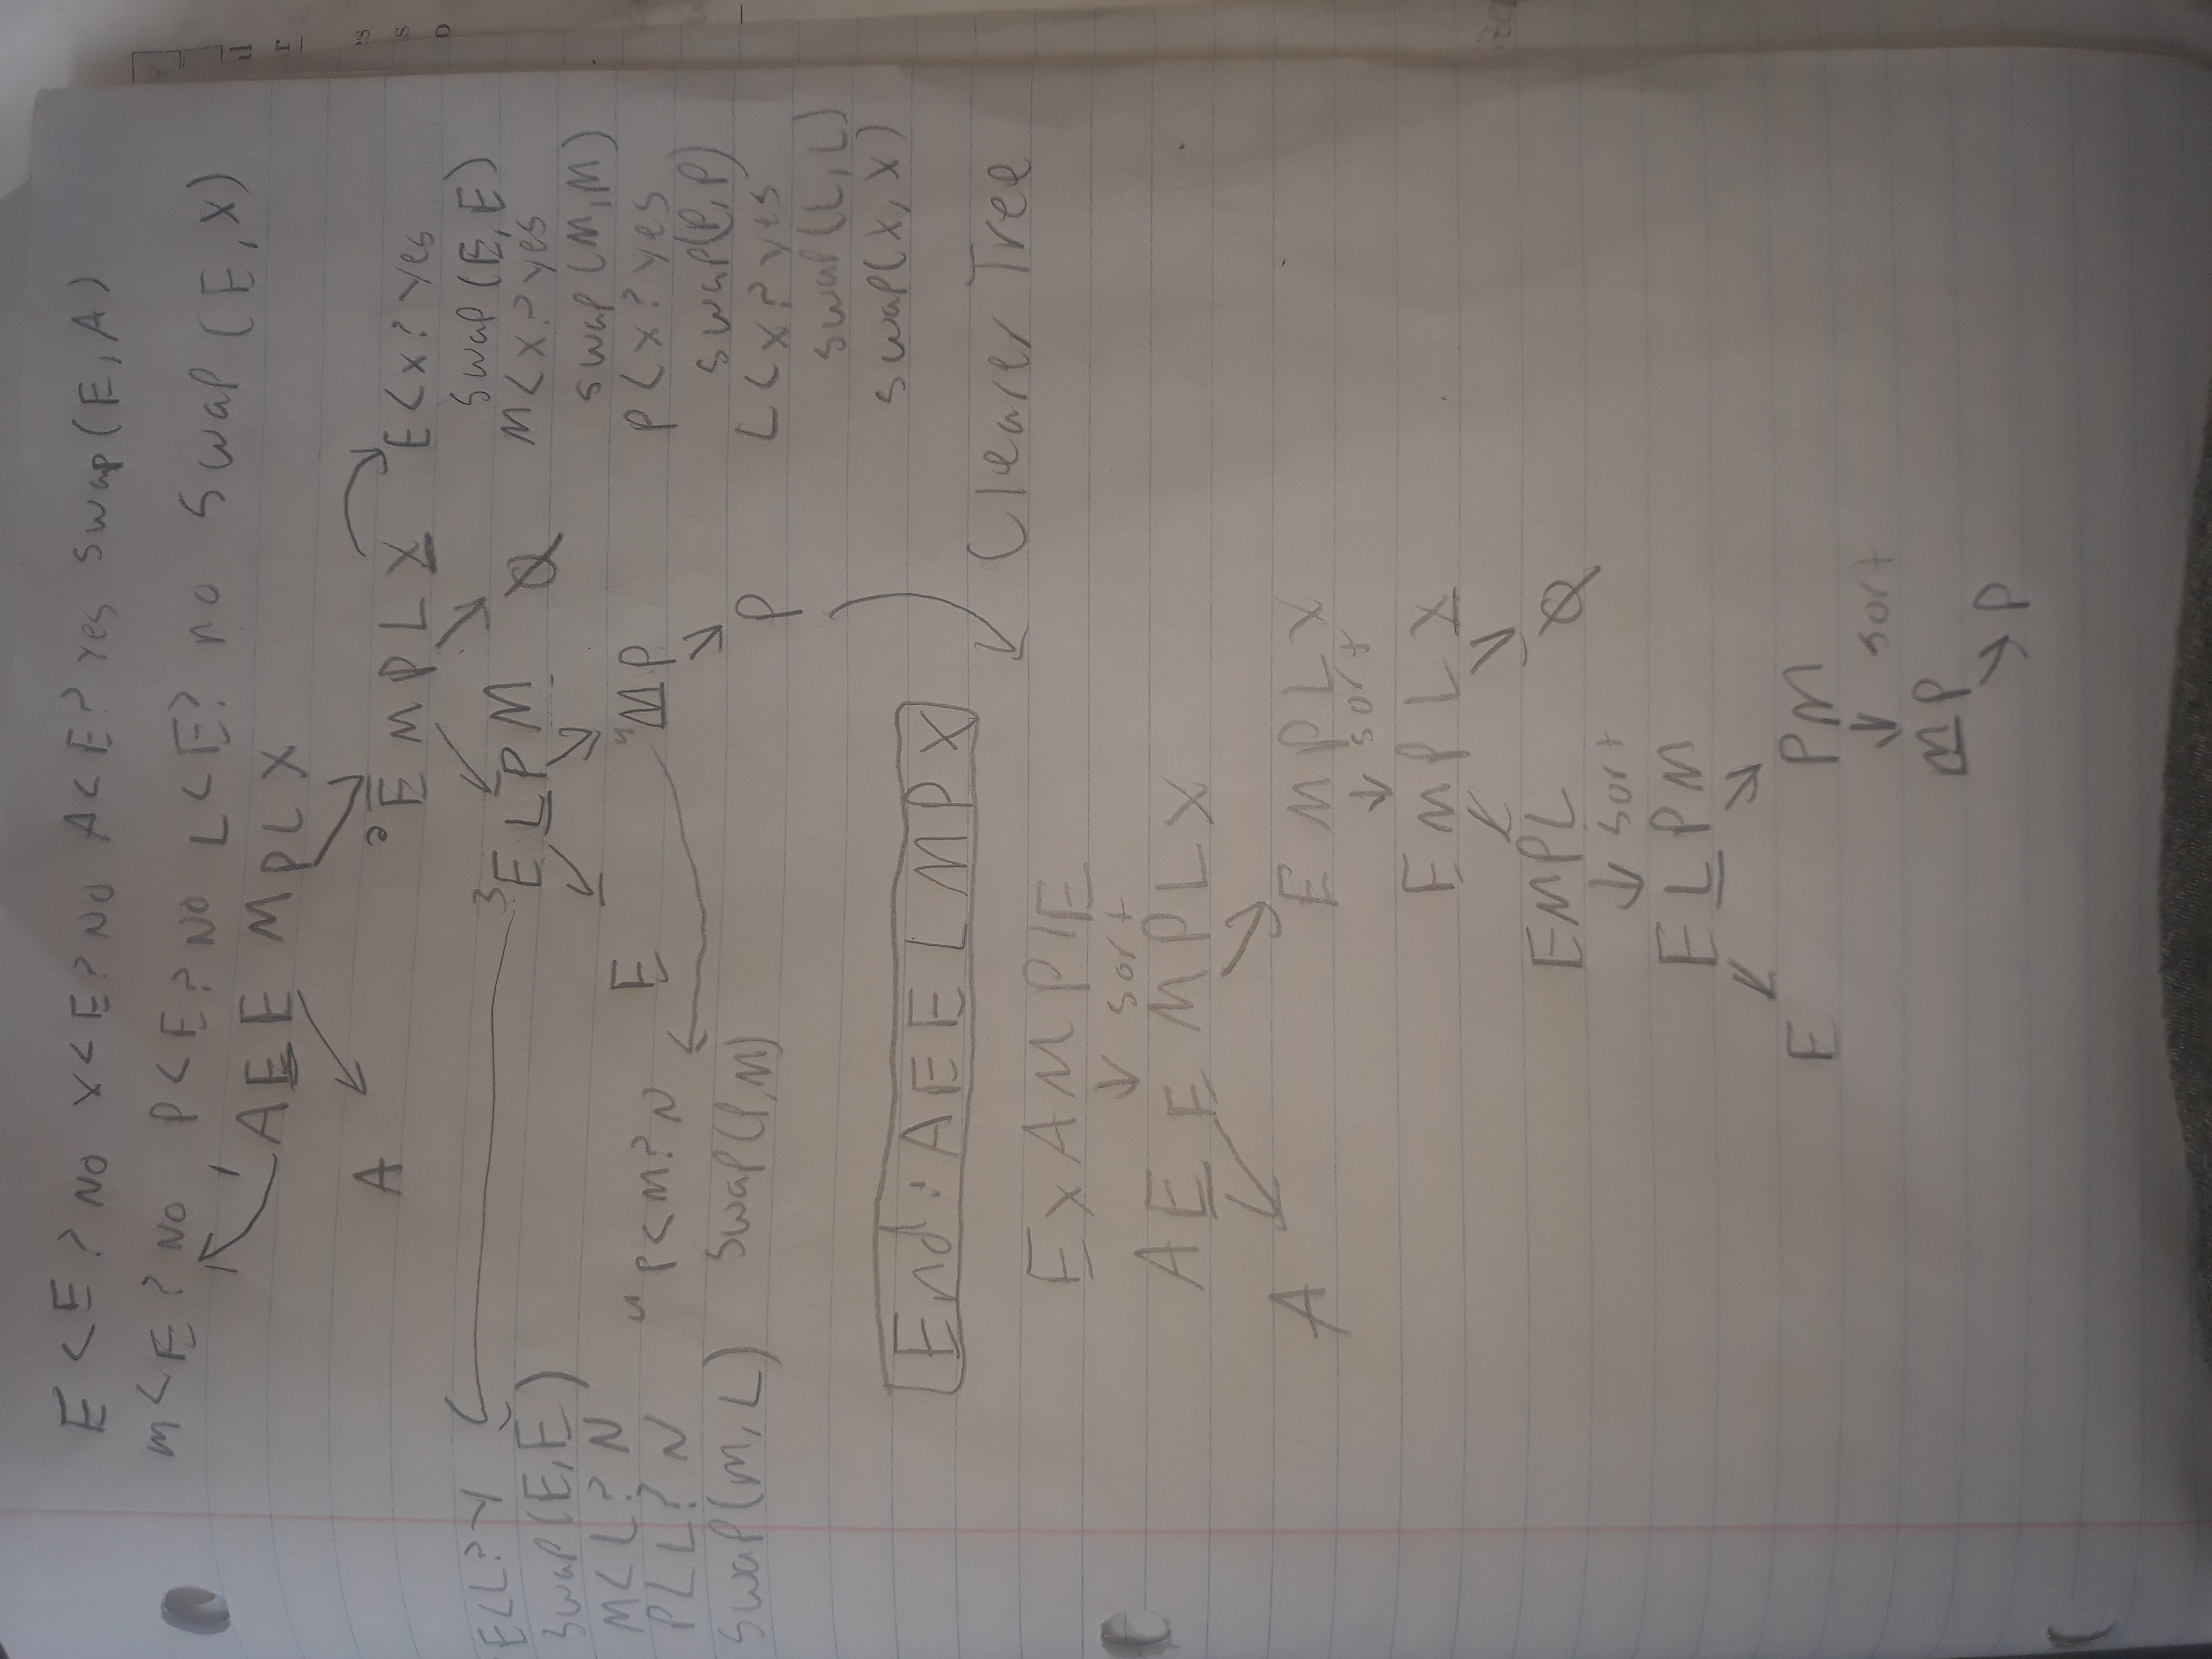
\includegraphics[width=\textwidth, angle=-90]{Quick}$ $\pagebreak$
    \end{solution}
	

    \item (6 pts) You are given a collection of $n$ bottles of different widths and $n$ lids of different widths and you need to find which lid goes with which bottle. You can compare a lid to a bottle, from which you can determine if the lid is larger than the bottle, smaller than the bottle, or the correct size. However, there is no way to compare the bottles or the lids directly to each other, i.e. you can't compare lids to lids or bottles to bottles. Design an algorithm for this problem with an average-case efficiency of $\Theta(nlgn)$
    
    \begin{solution}
        $\newline$ Quicksort(A,B,p,r): //A=array of lids, B= array of bottles $\newline -->$ if p$<$r: $\newline --/-->$ q=Partition(A,B,p,r) //Split the arrays  $\newline --/-->$ Quicksort(A,B,p,q-1) //Call sort on left side  $\newline --/-->$ Quicksort(A,B,q+1,r) //Call sort on right side $\newline$ End Basic Quicksort $\newline$ $\newline$ Partition(A,B,p,r): $\newline -->$ x=A[r] //Hold the last cap $\newline -->$ i=p-1 $\newline \newline -->$ //For loop using the cap to sort the bottles $\newline -->$   for j in range(p,r): //For the bottles $\newline --/-->$ if B[j] $\leq$ x: //If cap is too big/bottle too small $\newline --/--/-->$ i+=1 $\newline --/--/-->$ swap(B[j],B[i]) //Bring the smaller bottles backward  $\newline -->$ swap(B[i+1],B[r]) //put the correct bottle in place $\newline \newline -->$ y=B[i+1] $\newline -->$ ni=p-1 $\newline \newline -->$ //For loop using the picked bottle to sort the caps $\newline -->$  for ew in range(p,r): //Checks if the caps are less/greater than the bottle picked$\newline --/-->$ if A[ew]!=x: //Blocks the previous cap $\newline --/--/-->$ if A[ew] $\leq$  y: //If the cap is too small for the center bottle $\newline --/--/--/-->$ ni+=1 $\newline --/--/--/-->$ swap(A[ew],A[ni]) //Cap is smaller, swap it backward$\newline \newline -->$ swap(A[ni+1],A[r]) //Bring the original cap to the right spot $\newline -->$ return i+1 //Return where these pivots were located
    \end{solution}
    
\end{enumerate}


\end{document}


